% !TeX spellcheck = it_IT
\newpage
\section{Modelli di dati}
Progettare una BD significa progettare la struttura dei dati e le applicazioni. Per farlo al meglio è fondamentale rappresentare in modo \textbf{astratto} e simbolico il dominio del discorso tramite la \textbf{modellazione}.
\begin{definition}[Modello astratto]
	Un modello astratto è la \textbf{rappresentazione formale} di idee e conoscenze relative ad un fenomeno tramite un \textbf{linguaggio formale} a seguito di una \textbf{interpretazione} soggettiva.
\end{definition}

\subsection{Ruoli}
I ruoli principali nella modellazione sono:
\begin{itemize}
	\item \textbf{Committente}: persona con l'esigenza
	\item \textbf{Progettista} o \textbf{analista}: crea un progetto concettuale
	\item \textbf{Programmatore}: sviluppano la BD e le applicazioni
	\item \textbf{DB Administrator}: gestisce gli utenti e il sistema
\end{itemize}

\subsection{Fasi}
Le fasi della progettazione sono:
\begin{enumerate}
	\item \textbf{Analisi dei requisiti}: definizione dei bisogni del committente
	\item \textbf{Progettazione concettuale}: traduzione dei requisiti in un progetto, struttura concettuale dei dati, dei vincoli e delle operazioni
	\item \textbf{Progettazione logica}: traduzione dello \textit{schema concettuale} nello schema logico, che è espresso nel modello dei dati del sistema scelto
	\item \textbf{Progettazione fisica}: produce lo schema fisico che arricchisce quello logico con specifiche sull'organizzazione fisica dei dati
\end{enumerate}

\begin{center}
	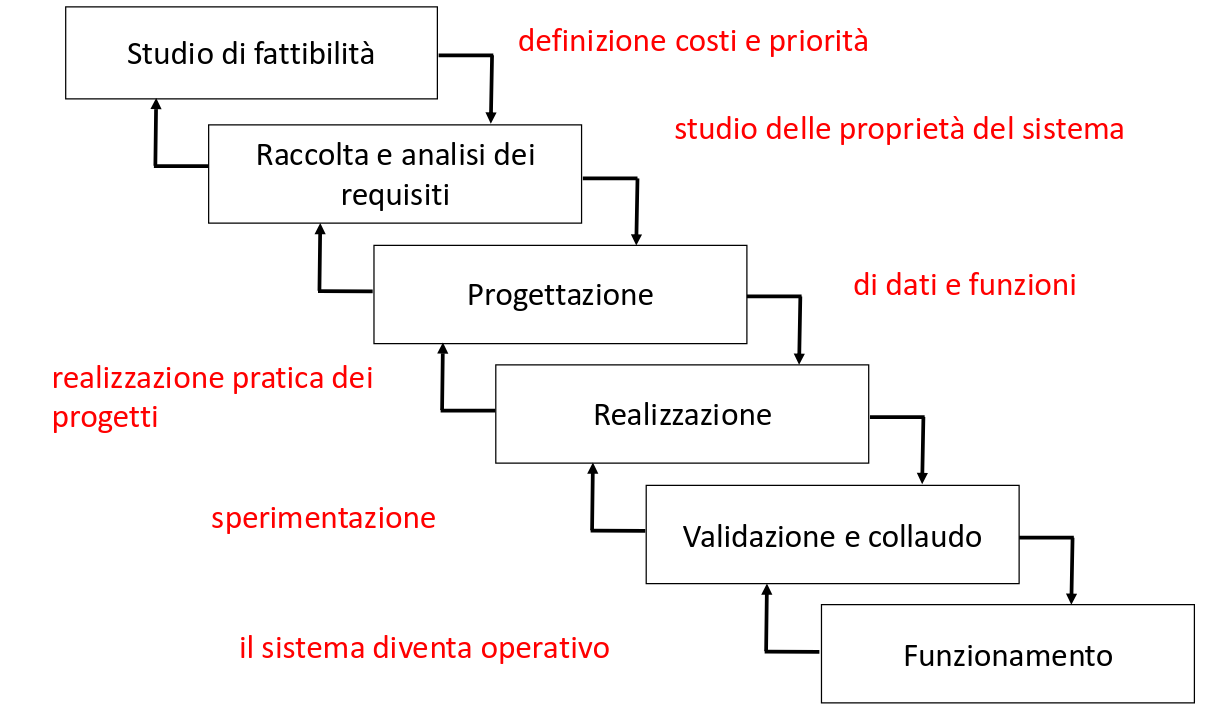
\includegraphics[scale=0.3]{fasi_prog.png}
\end{center}

\subsection{Aspetto ontologico}
Questo aspetto si concentra su quale conoscenza del dominio deve essere rappresentata. In particolare la conoscenza può essere \textbf{astratta}, \textbf{concreta} o \textbf{procedurale} (operazioni di base e comunicazione). 

\subsubsection{Conoscenza concreta}
La conoscenza concreta riguarda i \textbf{fatti} specifici che si vogliono rappresentare: \textbf{entità}, \textbf{collezioni} e \textbf{associazioni}.

\paragraph{Entità e proprietà}
Le \textbf{entità} sono ciò di cui ci interessa rappresentare alcuni fatti o proprietà (e.g. un libro) mentre le \textbf{proprietà} sono fatti che descrivono caratteristiche di determinate entità (e.g. titolo).

\begin{note}
	Un'entità non coincide con l'insieme dei valori assunti dalle sue proprietà, in quanto queste possono cambiare nel tempo o possono essere identiche pur essendo due entità diverse. E.g. una persona la cui età aumenta ogni anno o due persone con stesso nome, età e indirizzo.
\end{note}

Una \textbf{proprietà} è una coppia \textit{nome} e \textit{valore}, dove quest'ultimo è di un certo tipo e all'interno di un \textbf{dominio} di possibili valori. Si possono classificare come:
\begin{itemize}
	\item \textbf{Atomica} se il suo valore non è scomponibile, altrimenti \textbf{strutturata}
	\item \textbf{Univoca} se il suo valore è unico, altrimenti \textbf{multivalore}
	\item \textbf{Totale} o \textbf{obbligatoria} se ogni entità nell'universo assume un valore per essa, altrimenti \textbf{parziale} o \textbf{opzionale}
	\item \textbf{Costante} o \textbf{variabile}
	\item \textbf{Calcolata} o \textbf{non calcolata}
\end{itemize}

Un \textbf{tipo di entità} è una descrizione astratta di ciò che accomuna un insieme di entità omogenee, esistenti o possibili. È quindi un insieme infinito. E.g. persona, auto, esame.

\paragraph{Collezione}
Una collezione è un insieme \textbf{variabile} nel tempo di entità omogenee interessanti nel dominio. L'insieme degli elementi di una collezione in un dato momento è detto \textbf{estensione} della collezione. A differenza del \textit{tipo di entità}, questi insiemi sono finiti.

\paragraph{Associazione}

\begin{definition}[Istanza di associazione]
	Un'\textbf{istanza di associazione} è un fatto che correla due o più entità stabilendo un legame logico tra di loro. 
\end{definition}

\begin{definition}[Associazione]
	L'\textbf{associazione} $R(X,Y)$ fra due collezioni di entità $X$ e $Y$ è quindi l'insieme di istanze di associazione tra gli elementi di $X$ e $Y$ che varia nel tempo.
\end{definition}

\begin{definition}[Prodotto cartesiano]
	Il \textbf{prodotto cartesiano} $(X \times Y)$ è il dominio dell'associazione.
\end{definition}

\begin{observation}
	Se vediamo due collezioni $X$ e $Y$ come due insiemi, un’istanza di associazione tra di loro può essere vista come una coppia di elementi $(x; y)$, con $x \in X$ e $y\in Y$, e quindi un’associazione $R$ tra $X$ e $Y$ può essere vista come un sottoinsieme del prodotto $X \times Y$, ovvero come	una relazione matematica tra tali insiemi.
\end{observation}

\noindent Le associazioni hanno due caratteristiche strutturali:
\begin{itemize}
	\item \textbf{Molteplicità}
	\begin{definition}[Vincolo di univocità]
		Un’associazione $R(X, Y)$ è \textbf{univoca} rispetto ad $X$ se per ogni elemento $x \in X$ esiste al più un elemento di $Y$ che è associato ad $x$. Altrimenti è \textbf{multivalore} rispetto ad $X$.
	\end{definition}
	Questo ci porta alla \textbf{cardinalità} di un'associazione, che può essere:
	\begin{itemize}
		\item \textbf{Uno a molti}: $R(X,Y)$ è $(1:N)$ se essa è multivalore su $X$ ed univoca su $Y$
		\begin{center}
			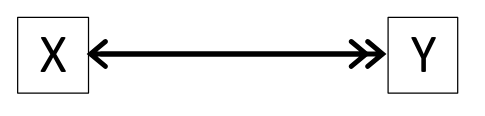
\includegraphics[scale=0.2]{unomolti.png}
		\end{center}
		\item \textbf{Molti a uno}: $R(X,Y)$ è $(N:1)$ se essa è univoca su $X$ e multivalore
		\begin{center}
			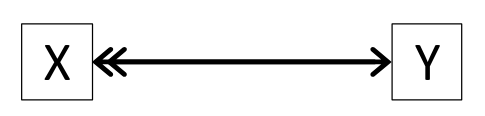
\includegraphics[scale=0.2]{moltiuno.png}
		\end{center}
		\item \textbf{Molti a molti}: $R(X,Y)$ è $(N:M)$ se essa è multivalore su $X$ e $Y$
		\begin{center}
			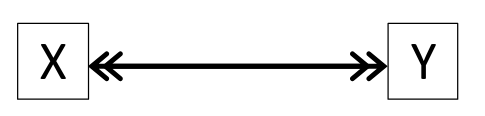
\includegraphics[scale=0.2]{moltimolti.png}
		\end{center}
		\item \textbf{Uno a uno}: $R(X,Y)$ è $(1:1)$ se essa è univoca su $X$ e $Y$
		\begin{center}
			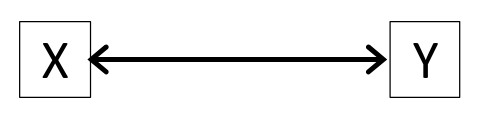
\includegraphics[scale=0.2]{unouno.png}
		\end{center}
	\end{itemize}
	\item \textbf{Totalità}
	\begin{definition}[Vincolo di totalità]
		Un’associazione $R(X, Y)$ è \textbf{totale} (o surgettiva) su $X$ se per ogni elemento $x \in X$ esiste almeno un elemento di $Y$ che è associato ad $x$. Altrimenti è \textbf{parziale} rispetto ad $X$.
	\end{definition}
	\begin{figure}[!h]
		\centering
		\begin{minipage}[b]{0.2\textwidth}
			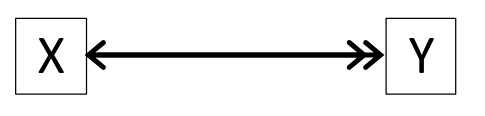
\includegraphics[width=\textwidth]{totale.png}
			\caption*{Totale}
		\end{minipage}
		\hspace{30pt}
		\begin{minipage}[b]{0.2\textwidth}
			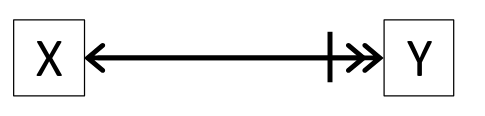
\includegraphics[width=\textwidth]{parziale.png}
			\caption*{Parziale}
		\end{minipage}
	\end{figure}
\end{itemize}

Un'associazione si rappresenta come visto e con l'aggiunta di un'\textbf{etichetta} con il suo nome, scelto di solito con un \textit{predicato}.

\subsubsection{Conoscenza astratta}
La conoscenza astratta riguarda i fatti generali che descrivono la \textbf{struttura} della conoscenza concreta, le \textbf{restrizioni} sui valori possibili della conoscenza concreta e sui \textbf{vincoli d'integrità} e le \textbf{regole} per dedurre nuovi fatti.

\begin{definition}[Modello dei dati]
	Un modello dei dati è un insieme di meccanismi di astrazione per descrivere la struttura della conoscenza concreta.
\end{definition}

\begin{definition}[Schema]
	Uno schema è la descrizione della struttura della conoscenza concreta e dei vincoli di integrità usando un particolare modello di dati.
\end{definition}

\begin{note}
	Come notazione grafica per lo schema usiamo una \textbf{variante} del modello ER.
\end{note}

\paragraph{Oggetti}
Ad ogni \textbf{entità} del dominio corrisponde un oggetto che può rispondere a dei \textbf{messaggi} (anche chiamati \textbf{attributi}), restituendo valori memorizzati o calcolati tramite procedure.

\begin{definition}[Oggetto]
	Un oggetto è un’entità software che	modella un’entità dell’universo e che ha:
	\begin{itemize}
		\item \textbf{Stato}: modellato da un insieme di costanti o variabili con valori di qualsiasi complessità
		\item \textbf{Comportamento}: un insieme di procedure locali chiamate \textbf{metodi}, che modellano le operazioni di base che riguardano l’oggetto e le proprietà	derivabili da altre
		\item \textbf{Identità}
	\end{itemize}
\end{definition}

\noindent Il \textbf{tipo oggetto} definisce l'insieme dei messaggi a cui può rispondere un insieme di possibili oggetti. Tra i tipi oggetto può essere definita una \textbf{relazione di sottotipo} che ha le seguenti proprietà:
\begin{itemize}
	\item È \textbf{asimmetrica}, \textbf{riflessiva} e \textbf{transitiva} (relazione di \textit{ordine parziale})
	\item \textbf{Sostitutività}: se $T$ è sottotipo di $T'$ allora gli elementi di $T$ possono essere usati in ogni contesto i cui possano apparire quelli di $T'$. In particolare:
	\begin{itemize}
		\item Gli elementi di $T$ hanno tutte le \textbf{proprietà} di quelli di $T'$
		\item Per ogni \textbf{proprietà} $p \in T'$, il suo tipo $T$ è un sottotipo del suo tipo in $T'$
	\end{itemize}
\end{itemize}

\paragraph{Classe}
Una classe è un insieme di oggetti dello stesso tipo, modificabile con operatori per includere o estrarre elementi dall'insieme.\\
Spesso le classi sono organizzate in una \textbf{gerarchia} di \textbf{specializzazione} o \textbf{generalizzazione} (\textbf{sottoclassi} e \textbf{superclassi}). Queste hanno due caratteristiche:
\begin{itemize}
	\item \textbf{Ereditarietà} delle proprietà che permette di definire:
	\begin{itemize}
		\item un tipo oggetto a partire da un altro
		\item l'implementazione di un tipo oggetto a partire da un'altra implementazione. In questo caso gli attributi possono solo essere \textbf{aggiunti} o \textbf{ridefiniti} solo specializzandone il tipo
	\end{itemize}
	\item Gli elementi di una sottoclasse sono un \textbf{sottoinsieme} di quelli della superclasse. Questa relazione ha le seguenti proprietà:
	\begin{itemize}
		\item È \textbf{asimmetrica}, \textbf{riflessiva} e \textbf{transitiva}
		\item \textbf{Vincolo intensionale}: se $C$ è sottoclasse di $C'$ allora il tipo degli elementi di $C$ è sottotipo degli elementi di $C'$
		\item \textbf{Vincolo estensionale}: se $C$ è sottoclasse di $C'$ allora gli elementi di $C$ sono un sottoinsieme degli elementi di $C'$
	\end{itemize}
\end{itemize}

I vincoli sugli insieme di sottoclassi possono essere di \textbf{disgiunzione} e di \textbf{copertura}. Questo porta ad avere quattro tipi di relazioni tra sottoinsiemi:
\begin{itemize}
	\item \textbf{Scorrelate}: non richiedono nessun vincolo e possono essere rappresentate in due modi
	\begin{center}
		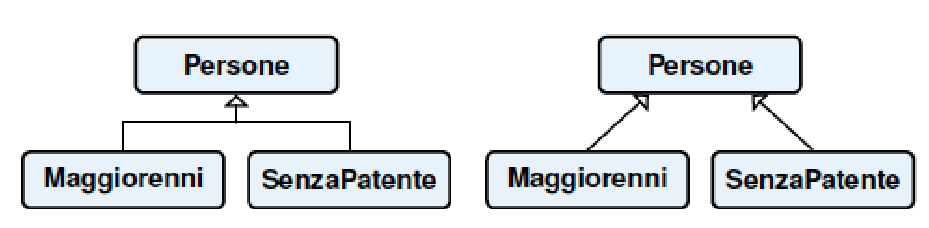
\includegraphics[scale=0.2]{scorrelate.png}
	\end{center}
	\item \textbf{Disgiunte}
	\begin{center}
		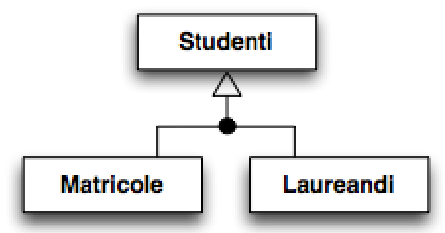
\includegraphics[scale=0.2]{disgiunte.png}
	\end{center}
	\item \textbf{Copertura}
	\begin{center}
		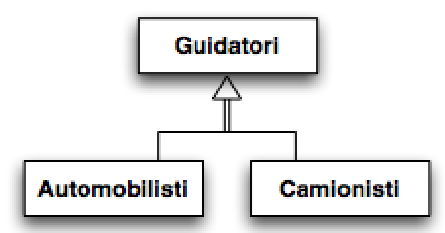
\includegraphics[scale=0.2]{copertura.png}
	\end{center}
	\item \textbf{Partizione}
	\begin{center}
		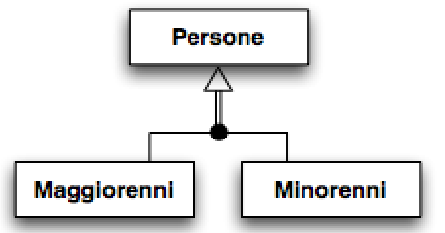
\includegraphics[scale=0.2]{partizione.png}
	\end{center}
\end{itemize}

È possibile avere l'\textbf{ereditarietà multipla} definendo un tipo per ereditarietà da più supertipi. Bisogna prestare attenzione quando un attributo viene ereditato da più antenati.

\paragraph{Associazioni}
Le associazioni si modellano con un costrutto apposito e possono avere delle \textbf{proprietà} ed essere \textbf{ricorsive}. L'ultimo caso si presenta quando abbiamo relazioni binarie fra gli elementi di una stessa collezione. In questo caso bisogna etichettare anche i ruoli agli estremi della freccia.
\begin{center}
	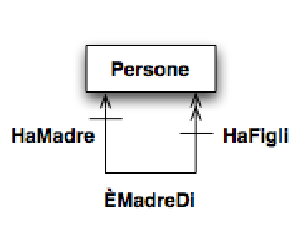
\includegraphics[scale=0.4]{ass_ric.png}
\end{center}
\begin{note}
	È possibile avere più associazioni tra classi diverse che rappresentano informazioni diverse.
\end{note}

\begin{observation}[Reificazione]
	È possibile trasformare un'associazione tra due classi in una situazione con tre classi e due associazioni. Ad esempio:
	\begin{center}
		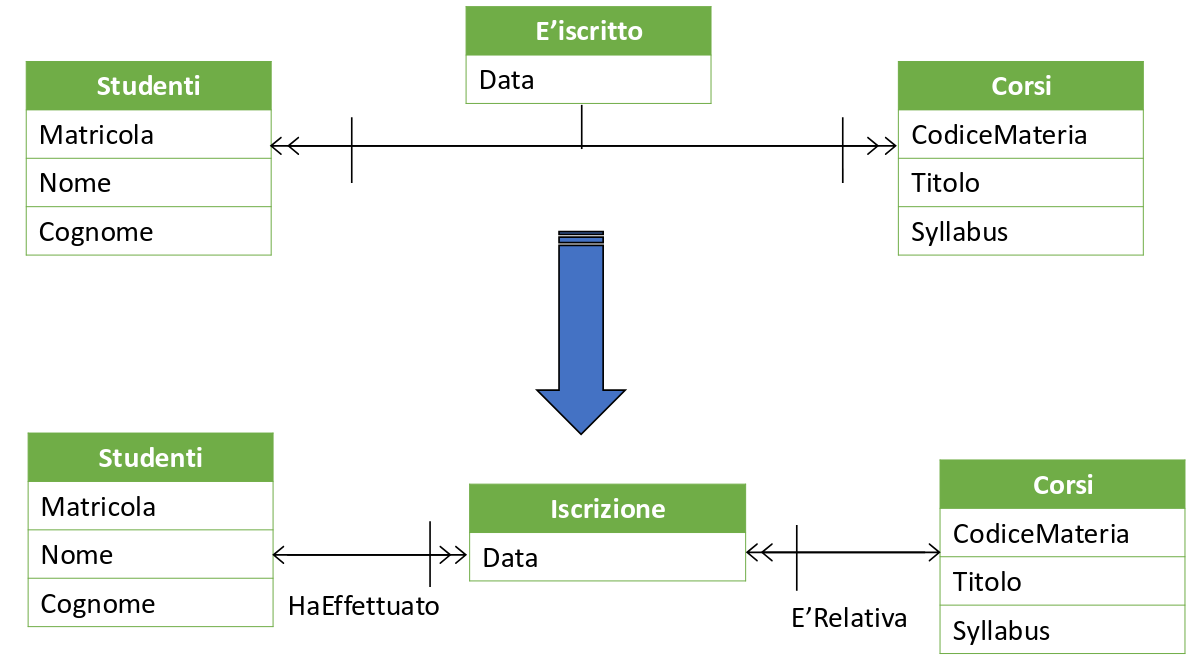
\includegraphics[scale=0.3]{reificazione.png}
	\end{center}
\end{observation}

\paragraph{Restrizioni}
I \textbf{vincoli d'integrità} impongono restrizioni sui possibili valori della conoscenza concreta. Possono essere \textbf{statici} o \textbf{dinamici} e arricchiscono la descrizione di una classe.
\begin{center}
	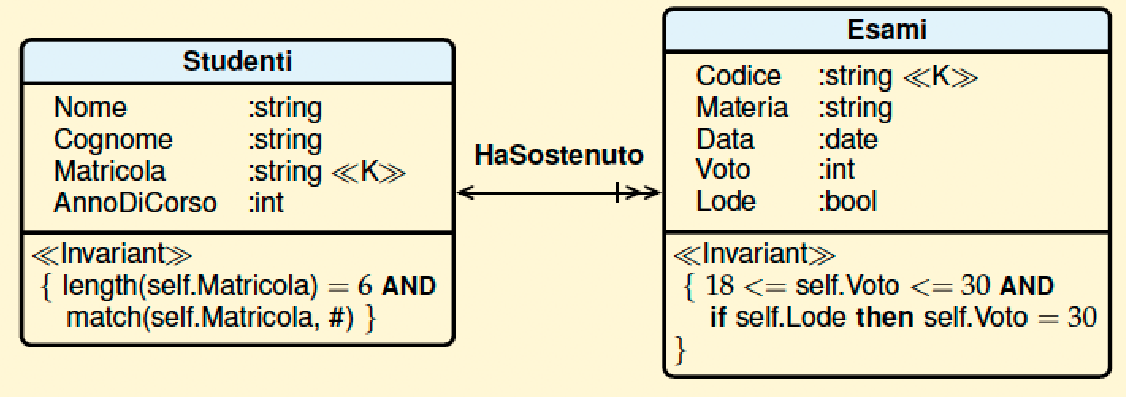
\includegraphics[scale=0.3]{vincoli.png}
\end{center}

\begin{note}
	Gli attributi marcati con $<<K>>$ sono una \textbf{chiave}.
\end{note}

\subsection{Modello entità-relazione}
È Il modello più popolare per il disegno concettuale di BD. Non tratta gerarchie di inclusione tra collezioni, non distingue collezioni e tipi e non supporta alcun meccanismo di ereditarietà. Definisce un meccanismo per modellare direttamente le associazioni non binarie o con proprietà.\\
Prevede due meccanismi di \textbf{astrazione}:
\begin{itemize}
	\item Modellare \textbf{insiemi di entità}, con le relative proprietà
	\item Modellare le associazioni (chiamate \textbf{relazioni}).
\end{itemize}
Le collezioni sono chiamate \textbf{tipi di entità}, e gli attributi dei loro elementi possono assumere solo valori di tipo primitivo.
\begin{center}
	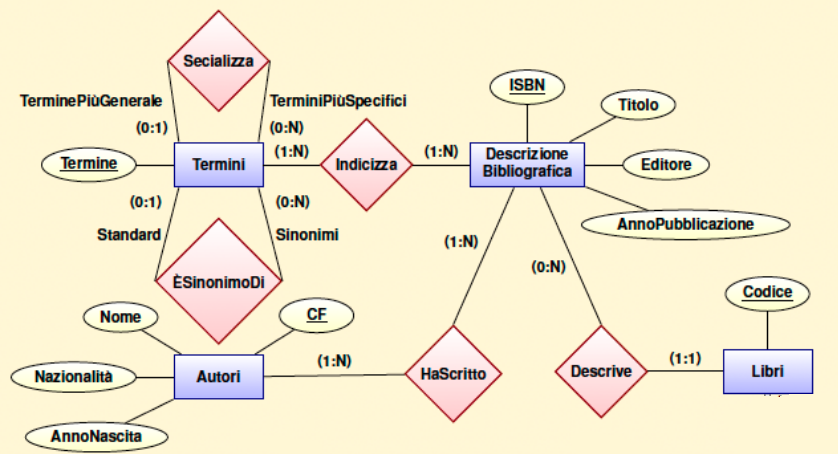
\includegraphics[scale=0.5]{entita_relazione.png}
\end{center}
\subsection{Modello relazionale}
E’ il modello dei dati usato dagli attuali sistemi commerciali. I meccanismi per definire una base di dati con questo modello sono l’\textbf{ennupla} e la \textbf{relazione}.

\begin{definition}[Ennupla]
	Un tipo ennupla è un insieme di coppie (attributo, tipo primitivo) ed un valore di tipo	ennupla è un insieme di coppie (attributo, valore), dette anche campi, con gli stessi attributi del tipo e in cui il valore di ogni attributo appartiene al corrispondente tipo	primitive.
\end{definition}

\begin{definition}[Relazione]
	Una relazione è un insieme di ennuple con lo stesso tipo.
\end{definition}

\begin{definition}[Superchiave e chiave]
	Un insieme di attributi i cui valori determinano univocamente un’ennupla di una	relazione $R$ è una \textbf{superchiave} per $R$. Una superchiave tale che togliendo un qualunque attributo essa non sia più una	superchiave è una \textbf{chiave} per $R$. Tra le chiavi di $R$ ne viene scelta una come chiave \textbf{primaria}.
\end{definition}
Le \textbf{associazioni} tra i dati sono rappresentate attraverso opportuni attributi, chiamati \textbf{chiavi esterne}, che assumono come valori quelli della chiave primaria di un’altra relazione. 

\begin{center}
	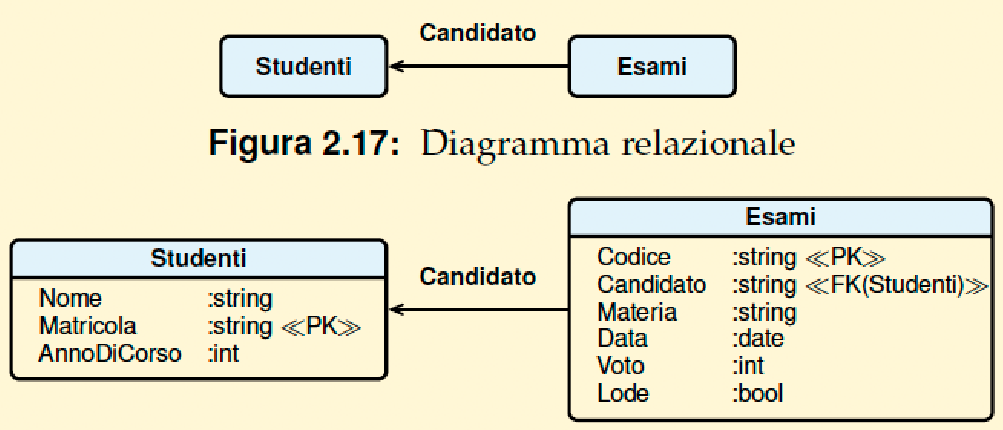
\includegraphics[scale=0.4]{mod_rel.png}
\end{center}